%!TEX TS-program = Arara
% arara: pdflatex: {shell: yes}
% Relative Koordinaten
\documentclass[12pt,ngerman]{scrartcl}

\usepackage{tikz}

\begin{document}

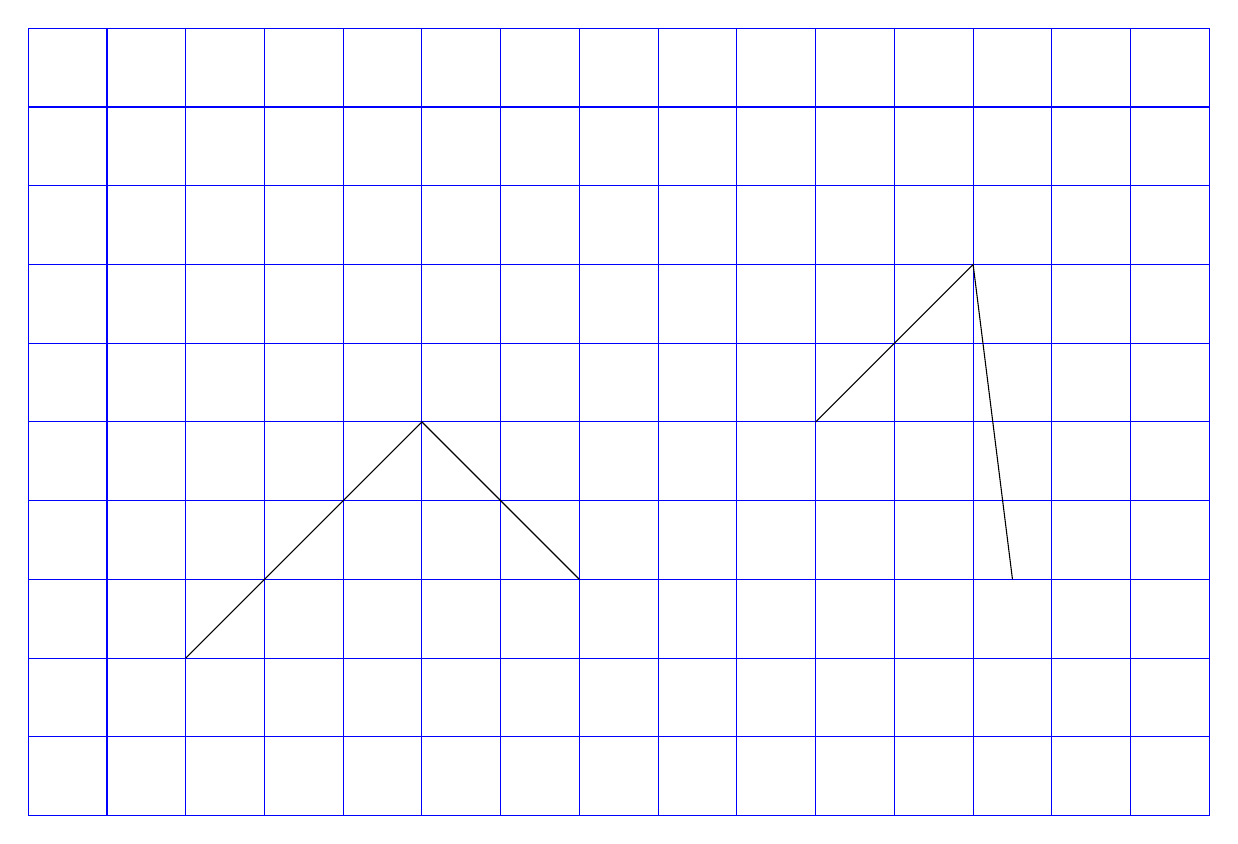
\begin{tikzpicture}
\draw[step=1cm, blue, thin](0,0) grid (15,10);

\draw(2,2) -- ++ (3,3) -- ++(2,-2); % Mit Update der Coordinate

% Ausgehend von 10,5 zeichne Linie nach +2,+2
% Ausgehend von 10,5 zeichne die Linie von 12,7 nach +2.5,-2
\draw(10,5) -- +(2,2) -- +(2.5,-2);

\end{tikzpicture}

\end{document}
